% DRAFT — arXiv preprint. Numbers in Section 5 are regenerated by
% research/vjepa-surprise/scripts/analyze_runs.py from results/ (see README).
% Search for TODO before submission.
\documentclass[11pt]{article}

\usepackage[margin=1in]{geometry}
\usepackage[utf8]{inputenc}
\usepackage[T1]{fontenc}
\usepackage{amsmath,amssymb}
\usepackage{booktabs}
\usepackage{graphicx}
\usepackage{xcolor}
\usepackage[numbers]{natbib}
\usepackage[hidelinks]{hyperref}

\newcommand{\todo}[1]{\textcolor{red}{[TODO: #1]}}

\title{Signal Temporal Logic over World-Model Latents:\\
Calibrated, Anticipatory Safety Monitoring at the Edge}

\author{\todo{authors and affiliations}}
\date{\todo{date}}

\begin{document}
\maketitle

\begin{abstract}
Edge safety monitors for mixed pedestrian--vehicle spaces typically reason over
geometry alone: detected objects, metric distances and velocities. Signal
Temporal Logic (STL) turns these into a quantified robustness margin, but the
margin is blind to what geometry cannot express---intent, unusual motion,
hazards outside the detector's vocabulary. We add a second kind of signal:
the \emph{surprise} of a self-supervised video world model, V-JEPA~2.1, measured
as the error of its latent predictor on the next second of video. Surprise is
calibrated per camera with split-conformal prediction and enters the STL
monitor as an ordinary signal under a \emph{tighten-only} rule, so learned
components can raise but never lower the geometric safety level. On a recorded
car-park deployment (Jetson Orin NX, 291\,s, 8 warning episodes), the ViT-g
model's own predictor anticipates geometric warnings 2\,s ahead with AUROC
0.70 (95\% CI 0.55--0.84) without any task-specific training, where a pixel
frame-difference baseline is at chance (0.48). Same-time detection is no
better than frame differencing, and frame-level pooling is dominated by
near-field motion; dense surprise maps nevertheless localise distant
pedestrians, motivating pair-local pooling. \todo{update once the staged
near-miss set and pair-local pooling are in.}
\end{abstract}

\section{Introduction}
\label{sec:intro}

Fixed-infrastructure safety monitoring---car parks, warehouses, platform
edges---needs answers that are both early and explainable. A binary detector
alarm is neither. SafeEdge, the system this work builds on, evaluates STL
specifications over geometric signals on an edge GPU and reports a signed
robustness margin $\rho$ every frame~\citep{maler2004stl,donze2010robust,nickovic2020rtamt}.
Its blind spots are structural: geometry cannot tell a parked car from one
about to move, linear trajectory extrapolation cannot foresee a turn, and
hazards with no detector class produce no signal at all.

Joint-Embedding Predictive Architectures (JEPAs) learn to predict the
\emph{representation} of missing or future content rather than its
pixels~\citep{lecun2022path,assran2023ijepa,bardes2024vjepa}. Their prediction
error behaves like a violation-of-expectation signal: it rises on physically
implausible events~\citep{garrido2025intuitive}. V-JEPA~2.1~\citep{murlabadia2026vjepa21}
makes every patch token a strong feature, which yields a dense, per-patch
surprise map.

\paragraph{Contributions.}
\begin{enumerate}
  \item STL signals defined over world-model surprise, with a tighten-only
        composition rule that preserves the geometric monitor's guarantees
        (Section~\ref{sec:method}).
  \item Per-camera split-conformal calibration of the surprise threshold,
        giving a bounded false-alarm rate on calm footage.
  \item An evaluation protocol that separates \emph{concurrent} detection from
        \emph{anticipation} and controls for pixel motion with a frame-difference
        baseline (Section~\ref{sec:setup}).
  \item Results on recorded deployment footage, including the negative finding
        that frame-level pooling mostly measures near-field motion
        (Section~\ref{sec:results}).
\end{enumerate}

\section{Background}
\label{sec:background}

\paragraph{STL robustness.} \todo{Brief STL syntax and quantitative semantics;
past-time operators as used by RTAMT for online monitoring.}

\paragraph{JEPA and V-JEPA 2.1.} A context encoder $E_\theta$ embeds the
visible part of a clip; an EMA target encoder $E_{\bar\theta}$ embeds the full
clip; a predictor $P_\phi$ predicts target embeddings at masked positions
$\Delta_y$, trained with
\begin{equation}
  \mathcal{L} = \bigl\lVert P_\phi\bigl(E_\theta(x), \Delta_y\bigr)
                - \operatorname{sg}\bigl(E_{\bar\theta}(y)\bigr) \bigr\rVert_1 .
\end{equation}
V-JEPA~2.1 adds a dense predictive loss over all tokens, deep self-supervision
over four encoder levels, modality-specific tokenizers and scaling to
2B parameters~\citep{murlabadia2026vjepa21}, building on
V-JEPA~2~\citep{assran2025vjepa2}.

\section{Method}
\label{sec:method}

\paragraph{Surprise.} Each window is 16 frames sampled at 4\,fps (4\,s), the
V-JEPA training rate. The 3D patch embedding yields $8 \times 24 \times 24$
tokens. The first six temporal slices (3\,s) are context; the last two (1\,s)
are the target. For target patch $p$,
\begin{equation}
  s_{t,p} = \tfrac{1}{D}\bigl\lVert P_\phi\bigl(E(\text{ctx}), \Delta_{\text{tgt}}\bigr)_p
            - E(\text{clip})_p \bigr\rVert_1 ,
\end{equation}
averaged over the two target slices, with $E$ the four-level hierarchical
features. The window score is the 95th percentile over patches. Scores are
stamped at the window's last frame, so $s(t)$ is causal.

The released distilled ViT-B/L predictors output in their ViT-G teacher's
feature space and cannot be scored against their own encoder. For these
edge-sized models we fit a per-patch linear (ridge) forecaster from the last
context slice to the mean target slice on calm footage, and score
$1 - \cos(\hat{z}, z)$.

\paragraph{Calibration.} Given $n$ calm calibration windows (all geometric
levels SAFE), the threshold $\tau$ is the $\lceil (n+1)(1-\alpha) \rceil$-th
smallest score; for new calm windows exchangeable with the calibration set,
$P(s > \tau) \le \alpha$~\citep{vovk2005algorithmic,angelopoulos2021gentle}.

\paragraph{STL integration.} With $\hat s = s/\tau$,
\begin{align}
  \varphi_6 &: \max\bigl(d_{\min} - d_{\text{zone}},\; 1 - \hat s\bigr), \\
  \varphi_7 &: \lnot\, \mathbf{H}_{[0,k]}\,(\hat s > 1),
\end{align}
where $\mathbf{H}$ is past-time \emph{historically}. Learned signals may only
raise the intervention level; the geometric specifications remain a floor. If
the latest score is older than a staleness bound, $\varphi_6$ and $\varphi_7$
evaluate as satisfied and the monitor falls back to geometry alone.

\section{Experimental setup}
\label{sec:setup}

\paragraph{Data.} One 291\,s clip (2244 frames, true capture rate 7.7\,fps)
from a deployed SafeEdge unit (Jetson Orin NX, USB camera, car park), recorded
in July (southern-hemisphere winter). Replaying it through the unchanged edge
loop (YOLOv8s, ByteTrack, homography, STL) yields a per-frame trace with
8 WARNING-or-higher episodes and 340 fully calm 4\,s windows. Two minutes of
the same camera's live feed from November (spring) serve as independent fitting
data. \todo{add the staged near-miss session and a public set, e.g. DoTA~\citep{yao2022dota}
or Street Scene~\citep{ramachandra2020streetscene}.}

\paragraph{Metrics.} Because $\rho_1$ on this clip jumps from the no-pair
sentinel straight to violation when a pedestrian is detected near a vehicle,
lead time before the geometric alarm is not informative. We report
(i) \emph{concurrent} AUROC: score vs.\ ``window contains WARNING+''; and
(ii) \emph{anticipation} AUROC: among fully calm windows, score vs.\
``WARNING+ within the next $H$\,s'', $H \in \{2, 4\}$. Positives cluster in
episodes, so 95\% intervals use a block bootstrap (20\,s blocks, 2000
resamples). Windows used to fit a forecaster are excluded from every metric.

\paragraph{Scorers.} Pixel frame difference (no model); ViT-B persistence;
ViT-B ridge fitted on the clip itself; ViT-B ridge fitted on the November
footage and applied unchanged (cross-season); ViT-g with its own predictor.

\section{Results}
\label{sec:results}

\begin{table}[t]
\centering
\small
\begin{tabular}{lccccc}
\toprule
Scorer & Concurrent & Antic.\ 2\,s [95\% CI] & Antic.\ 4\,s [95\% CI] & ms/win \\
\midrule
Pixel frame difference     & 0.853 & 0.483 [0.34, 0.63] & 0.534 [0.39, 0.69] & 7 \\
ViT-B persistence          & 0.818 & 0.454 [0.31, 0.61] & 0.490 [0.41, 0.60] & 40 \\
ViT-B ridge, in-clip$^\dagger$ & 0.955 & --- & --- & 40 \\
ViT-B ridge, cross-season  & 0.850 & 0.619 [0.50, 0.74] & 0.596 [0.49, 0.69] & 40 \\
\textbf{ViT-g predictor}   & 0.888 & \textbf{0.697 [0.55, 0.84]} & 0.647 [0.47, 0.83] & 268 \\
\bottomrule
\end{tabular}
\caption{Surprise vs.\ geometric WARNING+ on the July clip. Timings on an
RTX 4090. $^\dagger$Fitting consumed most pre-episode calm windows, leaving
4 (2\,s) and 8 (4\,s) positives; its concurrent AUROC is partly in-sample.}
\label{tab:main}
\end{table}

\begin{figure}[t]
\centering
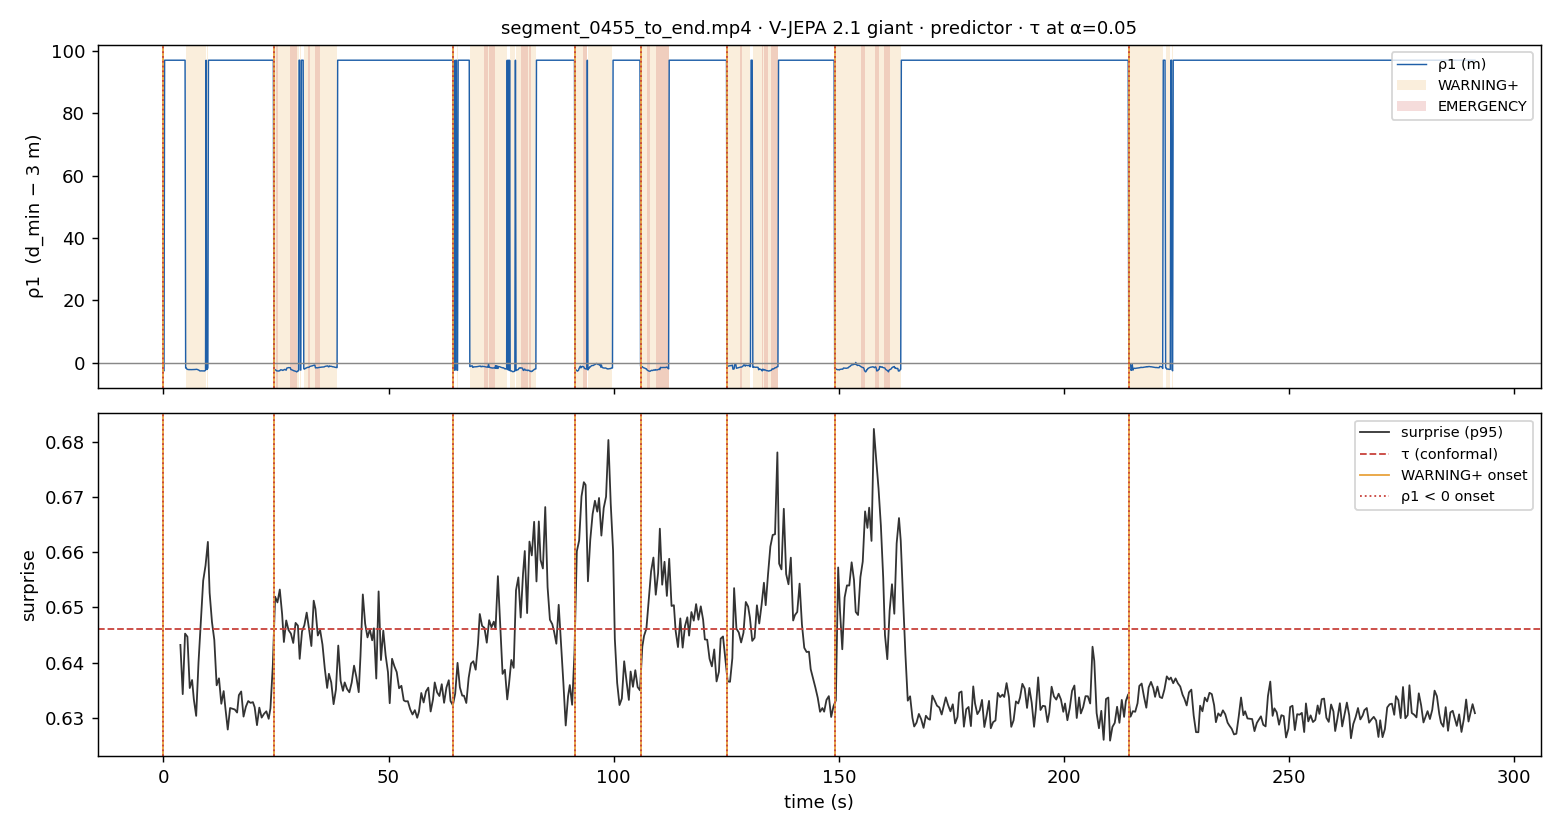
\includegraphics[width=\linewidth]{figures/vitg_predictor.png}
\caption{ViT-g predictor surprise (bottom) against $\rho_1$ and the geometric
intervention level (top). Orange lines: WARNING+ onsets; dashed: conformal
$\tau$ at $\alpha=0.05$.}
\label{fig:vitg}
\end{figure}

Table~\ref{tab:main} and Figure~\ref{fig:vitg} summarise the comparison.
Concurrent detection is comparable to frame differencing for every scorer:
during an episode, people and cars move, and anything sensitive to motion
fires. Anticipation separates the scorers. Both motion-only baselines are at
chance, the cross-season ridge forecaster is marginal, and the ViT-g
predictor's interval at 2\,s excludes 0.5.

\paragraph{Where the surprise is.} Inspecting the dense maps shows the largest
frame-level peaks come from a person walking close to the camera, not from the
pedestrian--vehicle pair. At the same time, the ViT-g map clearly marks a
distant pedestrian during a geometric warning that the frame-level score
misses. Restricting the score to far-field rows leaves the ViT-g anticipation
AUROC unchanged (0.70) while lifting the motion baselines only slightly, which
suggests the signal is not merely gross motion. \todo{figure: heat-map frames;
needs consent/anonymisation for publication.}

\section{Discussion and limitations}

\begin{itemize}
  \item \textbf{Scale of evidence.} Eight episodes from one clip and one camera.
        The anticipation effect needs confirmation on more events.
  \item \textbf{Pooling.} Frame-level pooling is dominated by near-field motion.
        Pooling around tracked pedestrian--vehicle pairs is the natural fix and
        uses geometry to aim the world model. \todo{results.}
  \item \textbf{Exchangeability.} The conformal guarantee assumes calm footage
        resembles calibration footage; lighting and season shift break this.
  \item \textbf{Compute.} ViT-g costs 268\,ms per window on a desktop GPU; the
        edge path needs distillation or the ViT-B route.
  \item \textbf{Detector variance.} The PyTorch replay produced 16 transitions
        where the deployed TensorRT build logged 23; all comparisons use one
        consistent trace.
\end{itemize}

\section{Conclusion}
\todo{One paragraph once pair-local pooling and the staged set are in.}

\paragraph{Reproducibility.} Code: \texttt{tools/vjepa\_surprise.py};
experiment record, per-window scores, surprise maps, trace and analysis:
\texttt{research/vjepa-surprise/} in \url{https://github.com/stanleyoz/safeEdge}.

\bibliographystyle{plainnat}
\bibliography{references}

\end{document}
